\subsection{Loaded DQL Migration During Pod Scale-Out}
\label{sec:live-dql-scaleout}

We next tested selective connection replacement during event delivery in a
separate Oracle Cloud cluster run. One client attached 1,000 registered
subscriptions to four persistent connections on one subscriber Pod, with
250 subscriptions per connection. The isolated deployment then grew from
one to four Ready Pods while the same client process remained running.
The second Pod became Ready before standby activation was released; the
third and fourth Pods were added during observation. The transport load
balancer assigned each empty probe to a Pod. The client used the retained
socket only when DQL selected migration and the execution guards passed.

The frozen checkpoint had 9,985 training updates and used $\epsilon=0$.
The trial allowed three executed actions in a configured 600-second window,
with a 60-attempt probe-discovery budget. Telemetry had to satisfy the
180-second age limit and 0.8 minimum backlog coverage. Each Pod requested
1.5 CPU cores and 4~GiB memory, with limits of three cores and 6~GiB.
The client used 32 workers and a fixed one-second processing delay to keep
work outstanding during handoff. This setting tests acknowledgement-aware
migration under a bounded client drain rate, rather than maximum Pod capacity.

Two bounded batches each published four synthetic source events. Each event
matched 5,000 registered subscriptions, including the client's 1,000-subscription
cohort. Thus, publication exposed the queue to 40,000 copies while the measured
cohort accounted for 8,000 delivery attempts. Capacity was checked before each
batch against the existing 400~MB limit, retaining an 80~MB reserve and prior
unreconciled publication costs. No queue purge or quota increase was used.

\begin{table}[!htbp]
  \centering
  \small
  \caption{Executed frozen-DQL handoffs in the loaded Oracle Cloud scale-out
  run. P1 is the initial Pod; P2 and P3 are added Pods. Drain time is included
  in total handoff time. These are three actions within one run.}
  \Description{Three handoffs each move 250 subscriptions and retain the other
  three active sessions. The first two move from P1 to P2; the third moves the
  first group again from P2 to P3. Total times are 97.555, 10.881 and 79.657 seconds.}
  \label{tab:live-dql-loaded-handoffs}
  \begin{tabular}{llrrrr}
    \toprule
    Action & Path & Subscriptions & Other sessions & Drain (s) & Total (s) \\
    \midrule
    H1 & P1 to P2 & 250 & 3 retained & 93.862 & 97.555 \\
    H2 & P1 to P2 & 250 & 3 retained & 8.339 & 10.881 \\
    H3 & P2 to P3 & 250 & 3 retained & 76.166 & 79.657 \\
    \bottomrule
  \end{tabular}
\end{table}

Table~\ref{tab:live-dql-loaded-handoffs} records actual policy execution, not
just a migration recommendation. The three observed differences between the
migration and stay Q-values were 1.7126, 1.2919 and 1.8201. Each migration was
admissible and selected by the frozen network. Before-and-after session maps
show that every handoff preserved the other three active connections. Two
original sessions remained unchanged throughout the run. The mechanism
therefore replaced selected connections without disconnecting the whole pool.

\begin{figure}[!htbp]
  \centering
  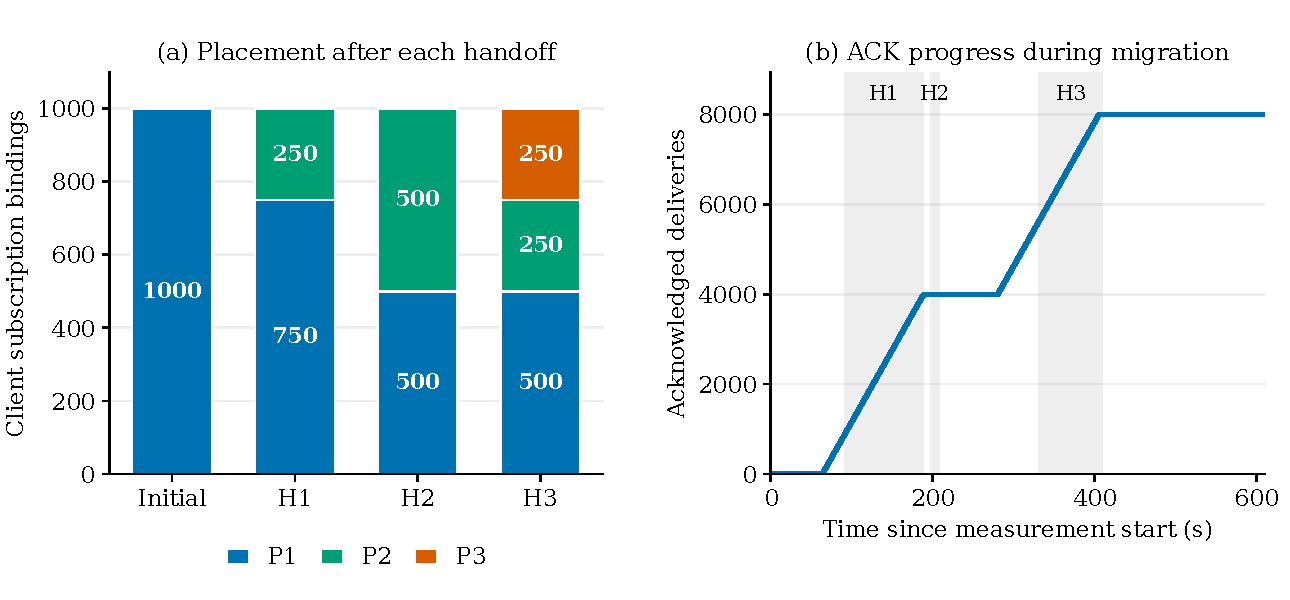
\includegraphics[width=\textwidth]{figures/live-dql-loaded-scaleout.pdf}
  \caption{Measured loaded DQL migration in the Oracle Cloud cluster.
  (a) Receipt-confirmed client bindings at the initial snapshot and after
  H1--H3. Each bar accounts for all 1,000 subscriptions; the four active
  connections each retain 250 subscriptions. P4 has no client bindings and
  is observed only through a probe. (b) Cumulative ACK receipts, aggregated
  in one-second bins. Shaded spans show the measured complete handoff
  intervals, including source drain. The curve describes this bounded
  workload, not a matched between-policy throughput comparison.}
  \Description{Placement changes from one thousand bindings on P1 to seven
  hundred fifty on P1 and two hundred fifty on P2, then five hundred on each,
  and finally five hundred on P1, two hundred fifty on P2 and two hundred fifty
  on P3. ACK receipts reach eight thousand while three shaded handoff intervals
  mark selective connection migration.}
  \label{fig:live-dql-loaded-scaleout}
\end{figure}

Figure~\ref{fig:live-dql-loaded-scaleout}(a) separates moved subscriptions
from handoff operations. H3 moves the group already transferred by H1, so
the three actions comprise 750 subscription-handoff operations involving
500 distinct subscriptions. The final distribution across the four available
Pods is 500, 250, 250 and zero. The maximum client population on one Pod falls
from 1,000 to 500, a 50\% reduction, without increasing the four active
connections. The last Pod remains a probe candidate after the three-action
budget is reached. Discovering it does not automatically promote it.

Figure~\ref{fig:live-dql-loaded-scaleout}(b) uses the confirmed ACK receipt
timestamp of each recorded delivery. Its cumulative total reaches 8,000,
and each of the 1,000 registered subscription hashes has eight acknowledged
delivery records. The ledger contains zero recorded ACK failures, processing
failures, duplicate candidates or unresolved deliveries at clean closure.
Long drain intervals remain visible: source retirement waits for outstanding
work instead of discarding it to shorten the measured handoff. The configured
window contains 60 decision records; its actual measurement boundaries span
609.716 seconds, including boundary handling.

The identity check uses STOMP message identifiers and confirms observed
delivery/ACK accounting. Source CloudEvent identities and individual backend
queue deletions are outside that ledger's scope. A separate unloaded
1,000-subscription run executed two handoffs in 5.244 and 5.172 seconds;
those timings are retained separately because the processing conditions
differ. The online and target weights remained identical to the input
checkpoint in both runs. The loaded run saved 39 valid experience transitions
without applying new training updates. The complete private archive verifies
256 files, and the manuscript figure uses identifier-free aggregates derived
from those records. The isolated deployment was restored to one Ready Pod;
all 13 shared-resource isolation checks passed.

\FloatBarrier
